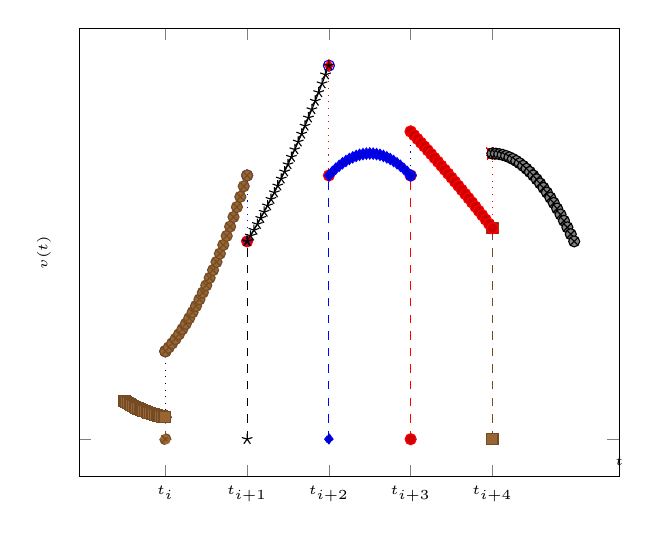
\begin{tikzpicture}
\begin{axis}[
		xtick = {0.1,.3,0.5,0.7,0.9},
		ytick = {0},
		x label style={at={(current axis.right of origin)},anchor=north, below=1mm},
		xlabel = {\tiny$t$},
		ylabel = {\tiny$v(t)$},
		yticklabels={},
		xticklabels={\tiny$t_{i}$,\tiny$t_{i+1}$,\tiny$t_{i+2}$,\tiny$t_{i+3}$,\tiny$t_{i+4}$}
]
\addplot+[mark=o,only marks] coordinates {(.1,.1) (.3,1.2) (.5,1.7) (.7,1.2) (.9,.96)};
\addplot+[mark=*,only marks] coordinates {(.1,.4) (.3,0.9) (.5,1.2) (.7,1.4) (.9,1.3)};
\addplot+[dashed] coordinates {(.1,0) (.1,.1)};
\addplot+[dashed] coordinates {(.3,0) (.3,.9)};
\addplot+[dashed] coordinates {(.5,0) (.5,1.2)};
\addplot+[dashed] coordinates {(.7,0) (.7,1.2)};
\addplot+[dashed] coordinates {(.9,0) (.9,.96)};

\addplot+[dotted] coordinates {(.1,.1) (.1,.4)};
\addplot+[dotted] coordinates {(.3,.9) (.3,1.2)};
\addplot+[dotted] coordinates {(.5,1.2) (.5,1.7)};
\addplot+[dotted] coordinates {(.7,1.4) (.7,1.2)};
\addplot+[dotted] coordinates {(.9,.96) (.9,1.3)};

\addplot+[solid,domain=.1:.3]{10*x*x+.3};
\addplot+[solid,domain=.3:.5]{5*x*x+.45};
\addplot+[solid,domain=.5:.7]{-10*(x-.6)*(x-.6)+1.3};
\addplot+[solid,domain=.7:.9]{-(x+.3)*(x+.3)+2.4};

\addplot+[dashed,domain=0:.1] {.1333 - x*.333 + 4*(x-.1)^2};
\addplot+[dashed,domain=.9:1.1] {1.3 - 10*(x-.9)*(x-.9)};	
\end{axis}
\end{tikzpicture}